\documentclass{article}

% Language setting
% Replace `english' with e.g. `spanish' to change the document language
\usepackage[english]{babel}

% Set page size and margins
% Replace `letterpaper' with `a4paper' for UK/EU standard size
\usepackage[letterpaper,top=2cm,bottom=2cm,left=3cm,right=3cm,marginparwidth=1.75cm]{geometry}

% Useful packages
\usepackage{amsmath}
\usepackage{graphicx}
\usepackage[table]{xcolor}
\usepackage[colorlinks=true, allcolors=blue]{hyperref}
\usepackage{tikz}
\usetikzlibrary{positioning}
\usepackage{enumitem}

\usepackage[
backend=biber,
style=ieee,
]{biblatex}


\addbibresource{sample.bib} %Imports bibliography file

\begin{document}

% ---------------------------
% Title page (custom)
% ---------------------------
\begin{titlepage}
  \begin{center}
    \includegraphics[width=5cm]{nup_logo.png} \\[1cm]
    {\Large Neapolis University Pafos} \\[0.5cm]

    \begin{tabular}{@{}l@{}}
      {\large \textbf{Course Code:} IS509} \\[0.2cm]
      {\large \textbf{Course Title:} Research Methodology} \\[0.2cm]
      {\large \textbf{Audience Instructor:} Marios Touloupos}
    \end{tabular} \\[2cm]

    {\huge \textbf{Final Project Assignment}} \\[1.5cm]

     \begin{tabular}{@{}l@{}}
      {\large \textbf{Name:} Aleksandr Petrunin} \\[0.3cm]
      {\large \textbf{Student ID:} 1251114137}
    \end{tabular} \\[2cm]

    {\large \today}
  \end{center}
\end{titlepage}

This project assignment constitutes a major component of IS509 and is designed to integrate the
theoretical and practical knowledge you acquire during the 13 weeks of lectures. The project will
allow you to demonstrate your ability to identify a research problem, conduct a literature review,
develop a conceptual framework, design an appropriate methodology, and critically analyze
findings.
\\\\
\textbf{Project Description:} You are required to develop a comprehensive research proposal or mini-
dissertation that addresses a clearly defined research problem in your field of interest. Your
project must demonstrate your understanding of research philosophies, literature review, theory
building, ethics, methodology design, data collection strategies, analysis, and presentation.
\\\\
\textbf{Deliverables:} Final Project Report: 3,500 – 5,000 words (excluding references, tables, and
appendices). Submission must be in Word or PDF format.
\\\\
\textbf{Assessment Criteria:} Your project will be assessed based on clarity, critical analysis, depth of
engagement with the literature, methodological rigor, originality, and academic writing quality.
This assignment is worth 20\% of your final grade.

\newpage
\tableofcontents
\listoftables
\listoffigures

\newpage
\begin{abstract}
 250-word abstract summarizing the study
\end{abstract}  

\section{Introduction}

\subsection{Background and context}

Goal: Establish research territory (broad academic landscape + demo knowledge of the field)\\
\textbf{Strategy:} Relevant + credible sources + historical context with current issues + balance depth and breadth.



\subsubsection{Broad context: Multi-agent systems with LLMs}
\subparagraph{}
The advancement of Large Language Models (LLMs) has ushered in 
a new era of autonomous AI agents capable of performing complex tasks 
with minimal human intervention \cite{yang2024llm}. Multi-agent systems (MAS) tend to outperform single-agent systems due to the larger pool of shared resources, coordination and specialization \cite{ye2025x}.
Businesses and individuals can leverage LLMs to build autonomous multi-agent systems with frameworks, such as AutoGPT,
CrewAI, and Langchain to automate workflows and optimize decision-making \cite{Sinha2025RiseOfMAS} \cite{Sinha2025BuildingMultiAgent} \cite{Chen2024PromiseOfMultiAgentAI}.



\subsubsection{Narrow focus: Agent-to-agent communication concepts and standards}
\subparagraph{}
However, current implementations of multi-agent systems predominantly rely on natural language processing (NLP) for inter-agent communication.
Agent-to-agent communication through natural language introduces several challenges, including ambiguity, misinterpretation, and inefficiencies in task execution \cite{zhou2025ai}.
A pool of protocols and orchestration mechanisms for structured communication between agents exists \cite{Yang2025SurveyAIProtocol}. 

\subparagraph{Older agent communication standards.} 
KQML (Knowledge Query and Manipulation Language) by DARPA is an early standard that provides a framework for knowledge sharing and querying among agents \cite{Finin1994KQML}.
FIPA Agent Communication Language (ACL) tried to cover KQML limitations and defines a set of communicative acts and message structures for agent communication \cite{inbook}. 

These languages found early adoption in academic, research, and experimental environments. They layed the foundation of modern software ecosystems, enabling everything from automated trading to smart home devices to work together \cite{DeRidder2024_SmythOS_ACLcomparison}.

However, FIPA-ACL and KQML were designed for symbolic AI systems with explicit knowledge representations. They are not so suitable for modern LLM-based agents that operate on distributed representations and natural language. 
Their fixed ontology requirements and predefined performative sets make them incompatible with the emergent behaviors of current multi-agent systems. 
On top of that, these languages lack of modern web protocol integration like HTTP, JSON, REST APIs. It might have prevented widespread adoption beyond research contexts.

\subparagraph{Current solutions.}
OpenAI Agents SDK is an orchestration mechanism, growing adoption in OpenAI ecosystem, not an inter-agent communication protocol \cite{OpenAI-Agents-Python}.
Model context protocol (MCP) by Anthropic provides a standardized way for AI models to connect with and use external tools and data sources - it is a client-to-agent protocol \cite{Anthropic2024_MCP}.

\subparagraph{Emerging standard.}
With ACP’s (protocol by IBM) recent merger into Google’s A2A (Agent to Agent) protocol under the Linux Foundation, A2A is rapidly becoming the dominant open standard for agent-to-agent communication \cite{LinuxFoundation2025_A2A}. 
In contrast to OpenAI Agents SDK, which provides only local IPC semantics, and the Model Context Protocol (MCP), which focuses on client-to-agent tool invocation, A2A is explicitly architected for distributed multi-agent systems. 
It defines message envelopes, routing, agent metadata, capability discovery, and extensible JSON-based interaction primitives. A2A and MCP are considered as complementary standards \cite{A2A2025}.

\newpage
\subsubsection{Specific gap: Semantic limitations of A2A protocol}
\subparagraph{}
Figure \ref{fig:semantic_gap} illustrates the communication landscape in multi-agent systems. 
Traditional formal protocols (FIPA-ACL, KQML) offered high semantic precision and verifiability. 
But they suffered from inflexibility and poor industry adoption. 
Modern LLM-based agents communicate through natural language prompts, planning steps, and role assignments. It provides adaptability, but also introduces ambiguity and non-determinism. 
Current standards like A2A provide syntactic infrastructure (message envelopes, routing, discovery) but lack semantic guarantees, leaving a gap. 
Our research targets this gap by proposing a typed semantic layer. This layer should bridge formal verification with LLM emergence behavior.

\begin{figure}[h]
\centering
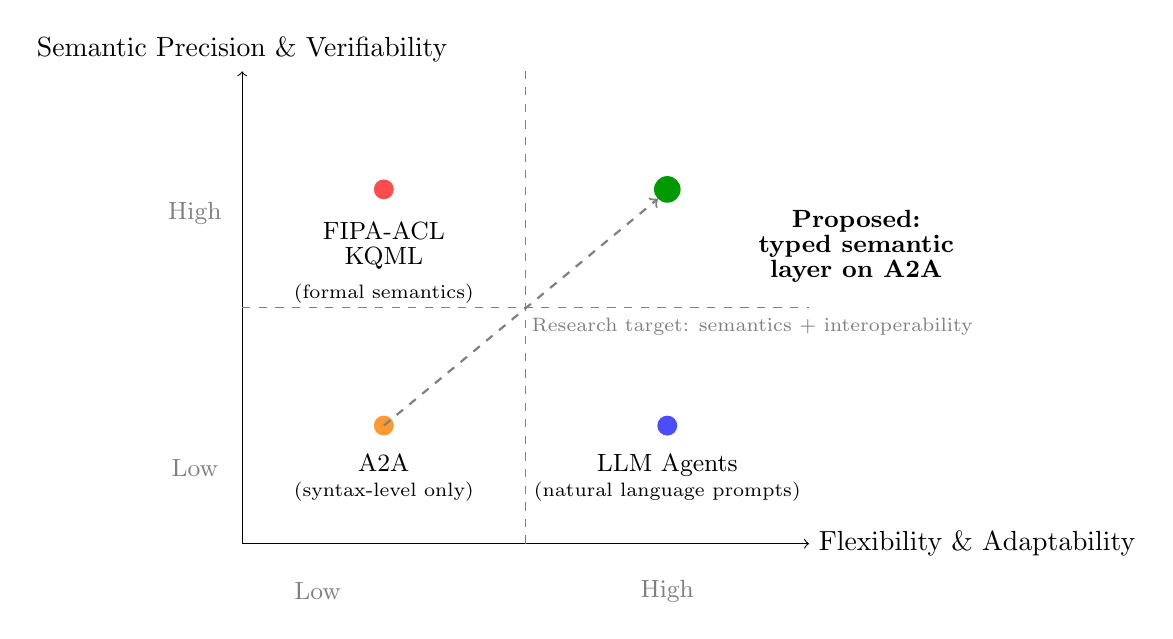
\begin{tikzpicture}[scale=1.2]
    % Axes
    \draw[->] (0,0) -- (6,0) node[right] {Flexibility \& Adaptability};
    \draw[->] (0,0) -- (0,5) node[above] {Semantic Precision \& Verifiability};

    % Grid lines
    \draw[gray, dashed] (0,2.5) -- (6,2.5);
    \draw[gray, dashed] (3,0) -- (3,5);
    
    % Quadrant labels (light gray)
    \node[text=gray, align=center] at (-0.5, 3.5) {\small High};
    \node[text=gray, align=center] at (-0.5, 0.8) {\small Low};
    \node[text=gray, align=center] at (0.8, -0.5) {\small Low};
    \node[text=gray, align=center] at (4.5, -0.5) {\small High};

    
    % FIPA-ACL / KQML (top-left quadrant center: high precision, low flexibility)
    \fill[red!70] (1.5, 3.75) circle (3pt);
    \node[align=center, font=\small] at (1.5, 3.15) {FIPA-ACL\\[-2pt]KQML};
    \node[font=\scriptsize, align=center] at (1.5, 2.65) {(formal semantics)};
    
    % A2A (bottom-left quadrant center: syntax only, no semantics)
    \fill[orange!80] (1.5, 1.25) circle (3pt);
    \node[align=center, font=\small] at (1.5, 0.7) {A2A\\[-2pt]\scriptsize (syntax-level only)};
    
    % LLM Natural Language (bottom-right quadrant center: high flexibility, low precision)
    \fill[blue!70] (4.5, 1.25) circle (3pt);
    \node[align=center, font=\small] at (4.5, 0.7) {LLM Agents\\[-2pt]\scriptsize (natural language prompts)};
    
    % Research contribution (top-right quadrant center: high precision + high flexibility)
    \fill[green!60!black] (4.5, 3.75) circle (4pt);
    \node[align=center, font=\small\bfseries] at (6.5, 3.15) {Proposed:\\[-2pt]typed semantic\\[-2pt]layer on A2A};
    
    % Arrow showing the gap
    \draw[->, dashed, thick, gray] (1.5, 1.25) -- (4.4, 3.65);
    \node[text=gray, font=\scriptsize, align=center] at (5.4, 2.3) {Research target: semantics + interoperability};
    
\end{tikzpicture}
\caption{Positioning of existing agent communication paradigms relative to semantic verifiability and adaptability.}
\label{fig:semantic_gap}
\end{figure}



\subparagraph{}
A2A protocol provides a much-needed open standard for agent interoperability. 
However, A2A standardizes only the syntax of communication: message envelopes, routing, and discovery. Unlike FIPA-ACL and KQML, which defined performatives and semantic frameworks, A2A does not prescribe message semantics, ontologies, shared meaning representations, or reasoning-level guarantees.
This semantic gap motivates research into typed, non-NLP communication layers that can enable more reliable, verifiable, and deterministic multi-agent behavior. We want to implement guarantees that agents understand each other beyond message structure.

\subsubsection{Solution: Typed semantic extension for A2A protocol}
\subparagraph{}
This research will develop a typed semantic extension for the A2A protocol that introduces formal performatives, interaction contracts, and verification constraints for multi-agent communication. 
We will leverage A2A's built-in extension mechanism (A2A Specification \href{https://a2a-protocol.org/latest/specification/#46-extensions}{Section 4.6}) 
to define strictly-typed message semantics inside the existing 'Message' metadata and extensions fields. 
The semantic layer will be implemented as an extension. It will be declared in Agent Cards and enable opt-in enforcement. At the same time backward compatibility will be preserved. 
We will prototype LLM-based MAS with this semantic layer and evaluate improvements in task reliability, negotiation consistency, and communication determinism. All three evaluation types will be compared to a baseline of natural-language-only A2A implementations.

\subsection{Statement of the problem}
Goal: Identify knowledge gaps(what remains unknown and unexplored $\to$ justify research).\\
LR $\to$ Gap analysis $\to$ problem statement/research aims.

\subparagraph{}
The A2A protocol, now the dominant open standard for agent-to-agent communication under the Linux Foundation, provides a comprehensive syntactic infrastructure but deliberately leaves semantic interpretation unspecified. The specification (Section 4.6) explicitly supports extensions for additional functionality, yet provides no guidance on semantic guarantees \cite{A2A2025}.

\subparagraph{Syntactic completeness without semantic guarantees.}
A2A defines three architectural layers: canonical data model (Task, Message, Artifact), abstract operations (Send Message, Get Task, etc.), and protocol bindings (JSON-RPC, gRPC, HTTP+JSON). However, the protocol intentionally adopts "opaque execution" as a guiding principle—agents collaborate based on declared capabilities without sharing internal reasoning or imposing semantic constraints on message interpretation \cite{A2A2025}.

\subparagraph{Concrete manifestations of the semantic gap.}
The absence of semantic layer results in:
\begin{enumerate}
  \item \textbf{No performatives:} Unlike FIPA-ACL (request, inform, query-ref), A2A provides no standard communicative acts. It forces agents to infer intent from natural language;

  \item \textbf{No interaction contracts:} Message exchange lacks pre/post-conditions or verification constraints. It results in weak formal validation of agent behavior;

  \item \textbf{No shared ontologies:} The protocol provides no mechanism for establishing common meaning representations;

  \item \textbf{Task state ambiguity:} A2A state transitions carry no semantic guarantees about what agents have agreed upon or accomplished.
\end{enumerate}

\subparagraph{Research questions.}
This gap raises critical questions: How can agents achieve deterministic communication within A2A's extension mechanism? What formal semantics are necessary for verifiable multi-agent coordination? Can a typed semantic layer maintain A2A's flexibility while enabling reliable task delegation and negotiation?

\newpage
\subsection{Justification of significance}
\textbf{Goal}: Present my contribution to the field, show how my research addresses these gaps and advance knowledge. \textbf{Strategy}: Magnitude + Urgency + Impact.

\subparagraph{}
This research addresses a gap in the emerging standard for agent-to-agent communication. 
A2A's explicit extension mechanism could provide a semi-standardized pathway for semantic enhancement, making this work potentially applicable to real-world deployments.

\subsubsection{Magnitude: Industry momentum and standardization urgency}
\begin{enumerate}[label=\alph*)]
  \item \textbf{Standard consolidation:} A2A emerged from the collaboration of Google's and IBM's competing protocols under Linux Foundation governanc. It is a signal of industry consensus on agent interoperability \cite{LinuxFoundation2025_A2A};

  \item \textbf{Enterprise readiness:} A2A's design principles explicitly target enterprise deployment with built-in authentication, authorization, asynchronous processing, and security considerations (Sections 7, 13);

  \item \textbf{Ecosystem growth:} Multi-agent frameworks (LangChain, AutoGPT, CrewAI) are adopting A2A as the interoperability layer;

  \item \textbf{Extension mechanism adoption window:} As A2A moves from draft (v1.0) to production.
\end{enumerate}

\subsubsection{Urgency: Real-world deployment challenges}
\textbf{Current state:} A2A agents communicate via natural language in Message.parts fields, relying on LLM interpretation without semantic constraints. This creates:
\begin{enumerate}[label=\alph*)]
  \item \textbf{Task coordination failures:} Agents misinterpret delegation intent in multi-turn interactions (contextId-linked tasks), leading to incorrect task state transitions;

  \item \textbf{Negotiation non-determinism:} Without formal performatives, agents cannot reliably establish commitments, preconditions, or mutual beliefs;

  \item \textbf{Prompt drift in long-running tasks:} A2A's async-first design supports tasks spanning hours or days, but semantic drift compounds over extended interactions;

  \item \textbf{Verification impossibility:} Enterprise deployments require audit trails and compliance verification, but natural language messages in Task.history cannot be formally validated.
\end{enumerate}

\textbf{Consequences of inaction:}
Production multi-agent systems will continue to exhibit unreliable behavior, limiting deployment to non-critical applications and preventing adoption in regulated industries (healthcare, finance, autonomous systems).

\subsubsection{Impact: Research and industry stakeholders}
\textbf{For researchers:}
\begin{enumerate}[label=\alph*)]
  \item Bridges formal agent communication theory (FIPA-ACL, KQML) with modern LLM-based agents;
  \item Provides empirical framework for evaluating semantic vs. syntactic protocol layers;
  \item Establishes methodology for protocol extension design within industry standards.
\end{enumerate}

\textbf{For industry practitioners:}
\begin{enumerate}[label=\alph*)]
  \item Immediate applicability: Semantic extension compatible with existing A2A implementations via Message.metadata and AgentCard.capabilities.extensions;
  \item Backward compatible: Agents without semantic support continue functioning, enabling gradual adoption;
  \item Enterprise value: Enables formal verification, audit trails, and compliance in regulated deployments.
\end{enumerate}
  
\textbf{For standardization bodies:}
\begin{enumerate}[label=\alph*)]
  \item Demonstrates practical use of A2A's extension mechanism for protocol evolution;
  \item Provides evidence-based guidance for potential inclusion in future A2A core specification;
  \item Establishes patterns for domain-specific semantic extensions in multi-agent ecosystems.
\end{enumerate}

\subparagraph{}
While this research primarily targets horizontal agent-to-agent communication, the semantic layer architecture may inform future work on client-to-agent protocols (MCP) and human-agent interaction, where precise intent interpretation is equally critical.

\newpage
\section{Literature review}
\newpage
\section{Research questions and hypotheses}
\newpage
\section{Methodology}
\newpage
\section{Expected findings and contributions}
\newpage
\section{Reflection and limitations}








\newpage
\printbibliography
\nocite{*}

\end{document}
